\documentclass[conference]{IEEEtran}
%\IEEEoverridecommandlockouts
% The preceding line is only needed to identify funding in the first footnote. If that is unneeded, please comment it out.
\usepackage{pgfplots}
\usepackage{array}
\usepackage{tabu}
\usepackage{hyperref}
\usepackage{subcaption}
\usepackage{cite}
\usepackage{amsmath,amssymb,amsfonts}
\usepackage{algorithmic}
\usepackage{graphicx}
\usepackage{textcomp}
\usepackage{xcolor}
\def\BibTeX{{\rm B\kern-.05em{\sc i\kern-.025em b}\kern-.08em
    T\kern-.1667em\lower.7ex\hbox{E}\kern-.125emX}}
\begin{document}

\title{Statistical  Analysis  of  Identity  Risk of Exposure  and  Cost  Using  the Ecosystem  of  Identity  Attributes
}

% \author{\IEEEauthorblockN{1\textsuperscript{st} Chia-Ju Chen}
% \IEEEauthorblockA{\textit{Center for Identity} \\
% \textit{University of Texas at Austin}\\
% ju40268@utexas.edu}
% \and
% \IEEEauthorblockN{2\textsuperscript{nd} Razieh Nokhbeh Zaeem}
% \IEEEauthorblockA{\textit{Center for Identity} \\
% \textit{University of Texas at Austin}\\
% razieh@identity.utexas.edu}
% \and
% \IEEEauthorblockN{3\textsuperscript{rd} K. Suzanne Barber}
% \IEEEauthorblockA{\textit{Center for Identity} \\
% \textit{University of Texas at Austin}\\
% sbarber@identity.utexas.edu}
% }

% \author{\IEEEauthorblockN{1\textsuperscript{st} ---}
% \IEEEauthorblockA{\textit{---} \\
% \textit{---}\\
% ---}
% \and
% \IEEEauthorblockN{2\textsuperscript{nd} ---}
% \IEEEauthorblockA{\textit{---} \\
% \textit{---}\\
% ---}
% \and
% \IEEEauthorblockN{3\textsuperscript{rd} ---}
% \IEEEauthorblockA{\textit{---} \\
% \textit{---}\\
% ---}
% }
\maketitle

\begin{abstract}
Personally Identifiable Information (PII) is often called the ``currency of Internet'' as identity assets are collected, shared, sold, and used for almost every transaction on the Internet.  PII is used for all types of applications from access control to credit score calculations to targeted advertising.  Every market sector relies on PII to know and authenticate their customers and their employees.   With so many businesses and government agencies relying on PII to make important decisions and so many people being asked to share personal data, it is critical to better understand the fundamentals of identity to protect it and responsibly use it.  Previously developed  comprehensive Identity Ecosystem utilizes graphs to model PII assets and their relationships and is powered by empirical data from almost 6,000 real-world identity theft and fraud news reports to populate the UT CID Identity Ecosystem. We obtained UT CID Identity Ecosystem from its authors to analyze using graph theory. We report numerous novel statistics using identity asset content, structure, value, accessibility, and impact.  Our work sheds light on how identity is used and paves the way for improving identity.
\end{abstract}

\begin{IEEEkeywords}
security and privacy, identity theft, graph theory, social network measures,  visualization
\end{IEEEkeywords}

\section{Introduction}
 Personally identifiable information (PII) is any data that could potentially be used to recognize a particular person, and it is commonly used in both physical and cyber spaces to perform personal authentication. Identity theft is the fraudulent acquisition and usage without permission of a person's PII. A modern authentication process usually requires collection of PII and increases the risk of exposure to identity theft and fraud criminals.

In 2017, the number of identity fraud victims increased by 8\% rising to 16.7 million U.S. consumers. Fraudsters stole from 1.3 million more victims in 2017 stealing a total of \$16.8 billion from U.S. consumers \cite{Pascual}. More intelligent and comprehensive approach should be provided to thwart the crime of identity theft.


In order to model the identity ecosystem, an intuitive  approach is to analyze the components from both cyber and physical aspects. Modern society  seamlessly merges online and offline PII attributes. Examples of on-line attributes are one's social media accounts, on-line shopping patterns, passwords, and email accounts. Off-line attributes are those related to the physical world such as bank accounts, credit and debit cards, Social Security Number, and one's physical characteristics.

 The UT CID Identity Ecosystem developed at the Center for Identity (CID) at the University of Texas (UT) at Austin constructed a graph-based model of people, devices, and organizations \cite{EcosystemModeling}. It models the relation as a Bayesian Network, and performs interference for possible sources of breaches and cost if the source is compromised.
It provides a framework for understanding the value, risk and mutual relationships for pairs of PII attributes. Each vertex represents an attribute whereas edges in-between imply the relationship.

For data source of ecosystem, The Identity Threat Assessment and Prediction (ITAP) \cite{ITAPDataSource} project is leveraged. ITAP is developed to focusing on gathering identity theft information from news stories, structuring this information, analyzing it, and discovering trends and characteristics.


We obtained UT CID Identity Ecosystem and the ITAP data source from their authors. Based on this graph-based network of identity, we have designed and implemented a visualization framework that facilitates understanding of the whole risk network rather than reviewing unstructured raw news feed data from ITAP. We introduce three main statistical evaluation criteria: (1) Traditional pie, bar, and scatter plots of vertex or edge specific values are employed to show the distribution. (2) Centrality measures such as degree, closeness, and betweenness centrality are introduced and hence illustrate each PII with certain structural features. (3) Strongly Connected Components (SCC) are applied to distinguish groups of PII that are interconnected.  With these criteria, our visualization framework can prototype the identity system with detailed features such as PII that are most efficient to spread the information if breached, or PII that are aggregated as a group that will easily be traversed if one member is already compromised. The main contribution of this paper includes the visual representation for the Ecosystem and the three criteria for modeling the identity ecosystem.  

The remainder of this article is structured as follow. Section II elaborates on the importance of statistical analysis of the Ecosystem tool and the set of measurements to be included. Section III presents a comprehensive evaluation and takeaways from the results. Section IV includes the related work of the identity ecosystem, identity theft, and related government reports. Section V concludes the research and gives insights for future work.

\section{Statistics Based on Ecosystem}

The Identity Ecosystem is a valuable previously implemented tool that models identity liaison, analyzes identity fraud and breaches, and answers several questions about identity risk management \cite{EcosystemModeling}. It maps identity attributes in a probabilistic model and performs Bayesian network-based inference to determine the posterior effects on each attribute. The Identity Ecosystem models individual identity attributes as nodes whereas edges in-between indicate various types of connections.
 
Each vertex includes different properties such as type of node, risk of exposure, and intrinsic monetary value. The Ecosystem Graphical User Interface (GUI) can color and size nodes based on their properties independently. Figure~\ref{fig:ecosystem_whole} shows an example snapshot in which the nodes are colored based on their risk of exposure and are sized based on their liability value.

\begin{figure}[ht]
  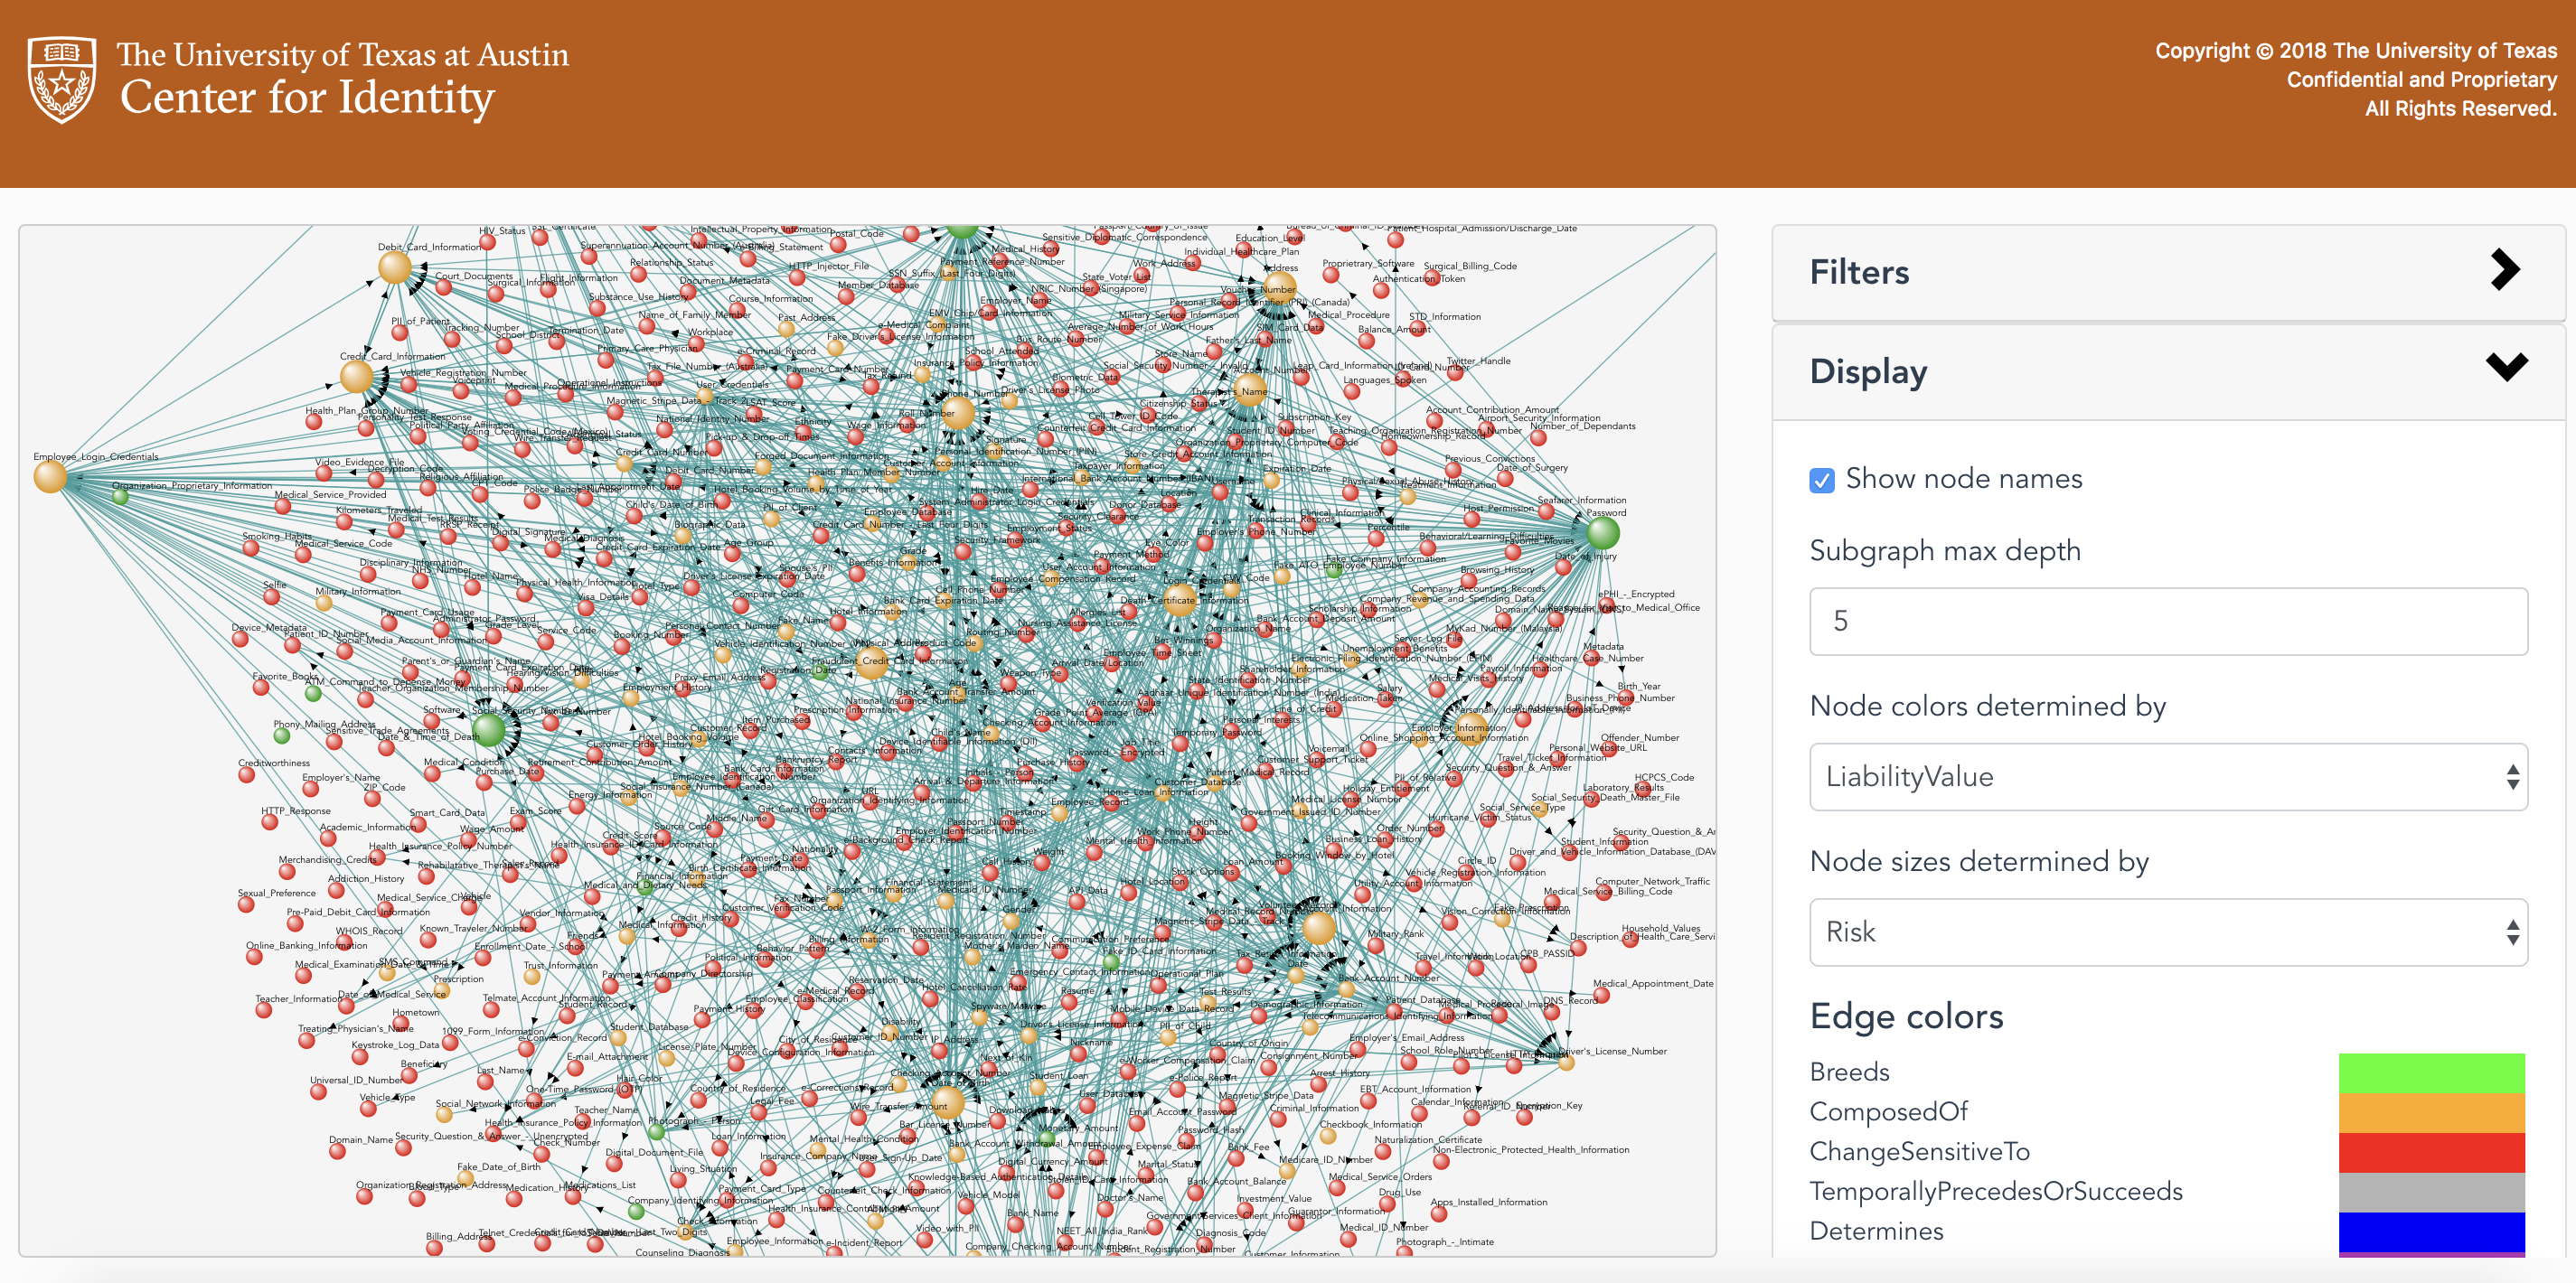
\includegraphics[width=\linewidth]{ecosystem_snapshot.png}
  \caption{Background: A snapshot showing previously developed  UT CID Ecosystem attribute graph.}
  \label{fig:ecosystem_whole}
\end{figure}

 The research questions we seek to answer in this paper are that ``In a graph-based network of identity, what are the underlying characteristics? Are PII forming groups or clusters? If so, what are the isolated PII nodes and connected ones?''. We would also want to answer ``Inside the network, which PII is in the critical path of obtaining others most often and which PII can influence the acquisition of the other PII?''. We further observe questions such as: ``In the PII graph, where is the PII located? Is it connected with lots of dangerous neighboring PII? Or is it placed on the boundary of a cluster?''.

We focus on three statistical indices on the given data set: (1) Bar, pie, and distribution charts based on the node or edge value (2) Centrality measurement including node specific in and out-degree centrality, betweenness centrality, and closeness centrality and (3) Strongly connected  components of nodes for identifying clusters. Based on the results, a comprehensive discussion is presented about possible breaches with more important attributes, and flow of personal information inside the network modeling the real-world information movement. 



\section{Statistical Charts}

We present sets of mathematical formula and statistical chart visualization in this section. The data source we used is from ITAP in Ecosystem, which contains 627 PII attributes in total. We divide the analyses based on edge or node specific properties. We represent the Identity Ecosystem as a graph $G(V, E)$ consisting of N attributes $A_{1}$, ...,$A_{N}$ and a set of directed edges as tuples $e_{ij} = \langle i, j \rangle$ where $A_{i}$ is the originating node and $A_{j}$ is the target node such that $1 \leq i, j \leq N$. Each edge $e_{ij}$ represents a possible path by which $A_{j}$ can be breached given that $A_{i}$ is breached. Each node $A_{j}$ is labeled with a Boolean random variable, denoted $D(A_{j})$, which is true if the attribute has been exposed and false otherwise. Each edge $e_{ij}$ represents a possible path by which $A_{j}$ can be breached given that $A_{i}$ is breached. For simplicity, we consider all edges to be independent. Therefore, we can assign conditional probabilities to each edge with $Prob(e_{ij}) = Prob(D(A_{j})|D(A_{i}))$.

\subsection{Statistical charts based on edges}
We implement the pie chart to observe the percentage for PII with/without outgoing edges or with/without incoming edges as shown in Figure~\ref{fig:pie_pii}. We can observe that 211 PII attributes (33\%) are with incoming edges, while 45 (7\%) are with outgoing edges.

{\bf Insight:} Only 7\% of PII have any effect on the risk of exposure of others and a total of 33\% could possibly be affected. The PII with outgoing edges should be carefully protected. The most important PII in this list are discussed shortly.

\begin{figure}[ht!]
  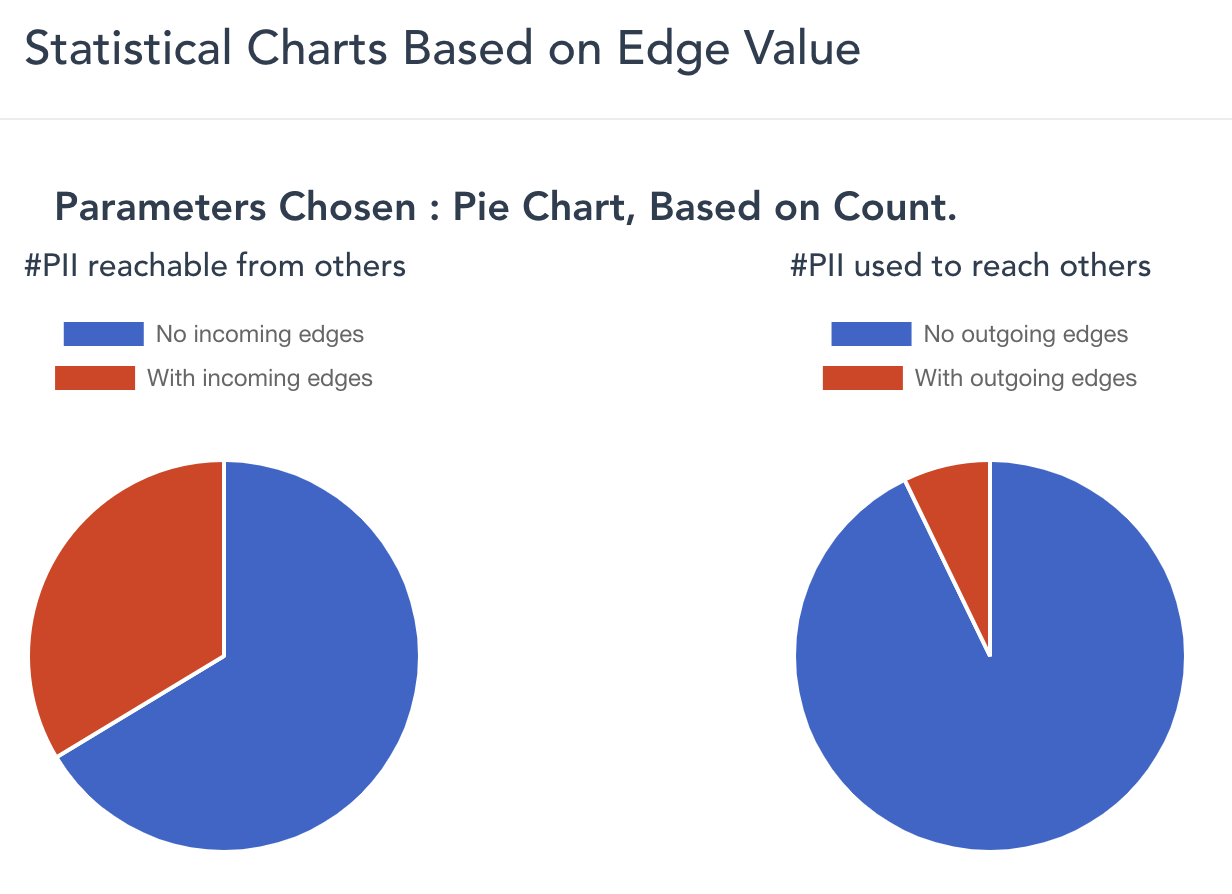
\includegraphics[width=\linewidth]{pie_PII.png}
  \caption{A snapshot showing pie charts for percentage of nodes with/without in/out degree.}
  \label{fig:pie_pii}
\end{figure}

% The Ecosystem predicts the risk (i.e., probability) of breach for a PII and a potential dollar value damage to the owner if a certain attribute is fraudulently used. We next focus on calculating degree centrality. 

 Furthermore, taking the probability on the edges into account, we extend the degree centrality from summing discrete edge count to accumulating risk.
Degree centrality equals the number of links that a vertex has with other vertices. The equation for this measure is as follows: 

\begin{equation}
C_{D_{out}}(v_i) = outdegree(v_{i}) = |\{e_{ij}\}|
\end{equation}
\begin{equation}
C_{D_{in}}(v_i) = indegree(v_{i}) = |\{e_{ji}\}|
\end{equation}

If we consider the weight (i.e., probability) on edges, this yields the equation:
\begin{equation}
C_{W_{out}}(v_i) = \Sigma Prob(e_{ij})
\end{equation}
\begin{equation}
C_{W_{in}}(v_i) = \Sigma Prob(e_{ji})
\end{equation}

Figure ~\ref{fig:barchart_most_count} presents the top 10 PII in descending order based on the number of incoming and outgoing edges. The top three attributes with the highest number of incoming edges, i.e., most easily discoverable through incoming edges, are \textit{Name}, \textit{Credit Card Information}, and \textit{Date of Birth}. Also, the top three attributes with the highest number of outgoing edges, i.e., most likely able to reach the wide variety of PII through outgoing edges, are \textit{Customer Database}, \textit{Password}, and \textit{Email address}. Figure~\ref{fig:barchart_most_weight} shows the same statistics on the top 10 PII with most incoming and outgoing edges, with the difference that it considers the sum of weights on the edges instead of merely the edge count.

{\bf Insight:} \textit{Name} has the highest rank among PII discoverable from others through incoming edges and \textit{Customer database} sits at the top of nodes with the highest outgoing degree, whether the edge count or edge weight is considered.

\begin{figure}[ht!]
  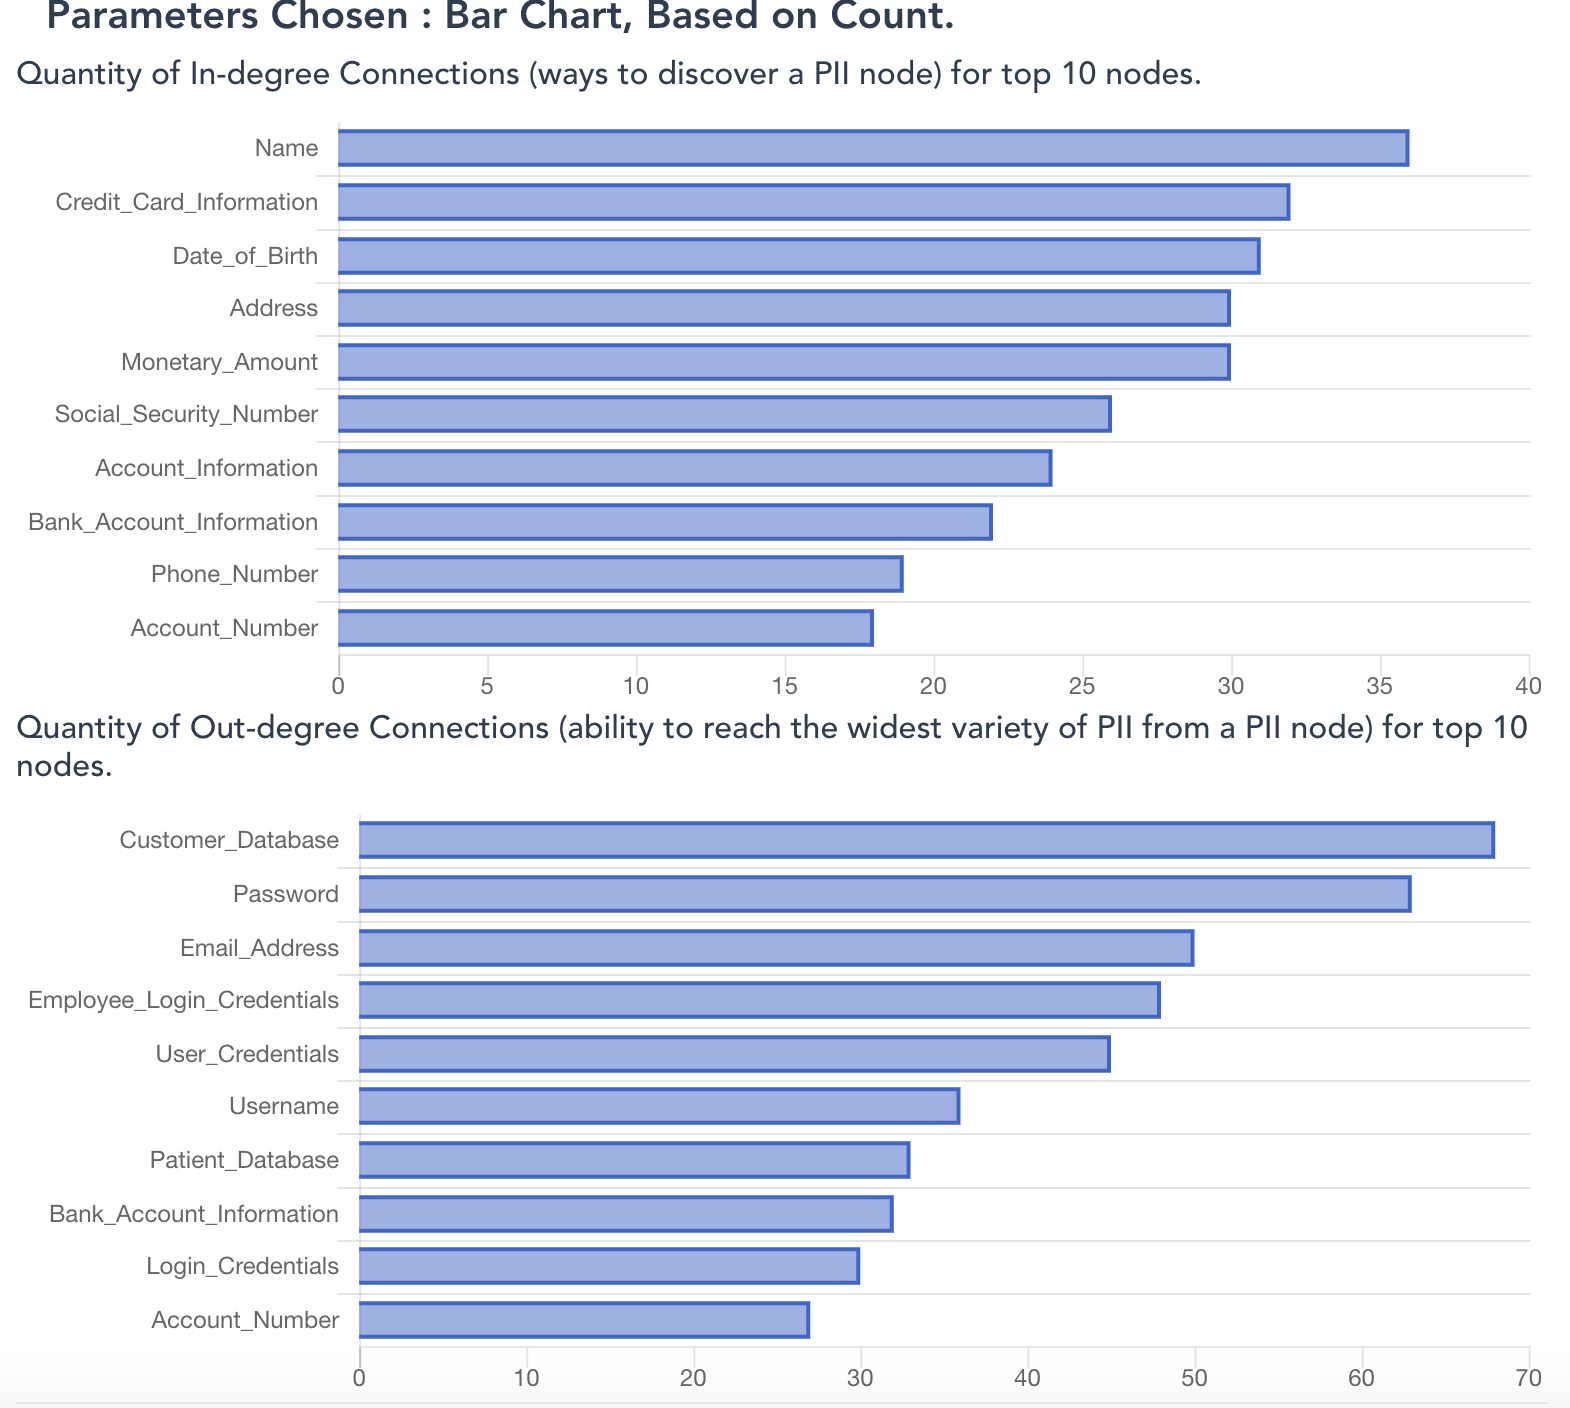
\includegraphics[width=\linewidth]{barchart_most_count.png}
  \caption{A snapshot showing top 10 PII with most in and out degree count.}
  \label{fig:barchart_most_count}
\end{figure}

\begin{figure}[ht!]
  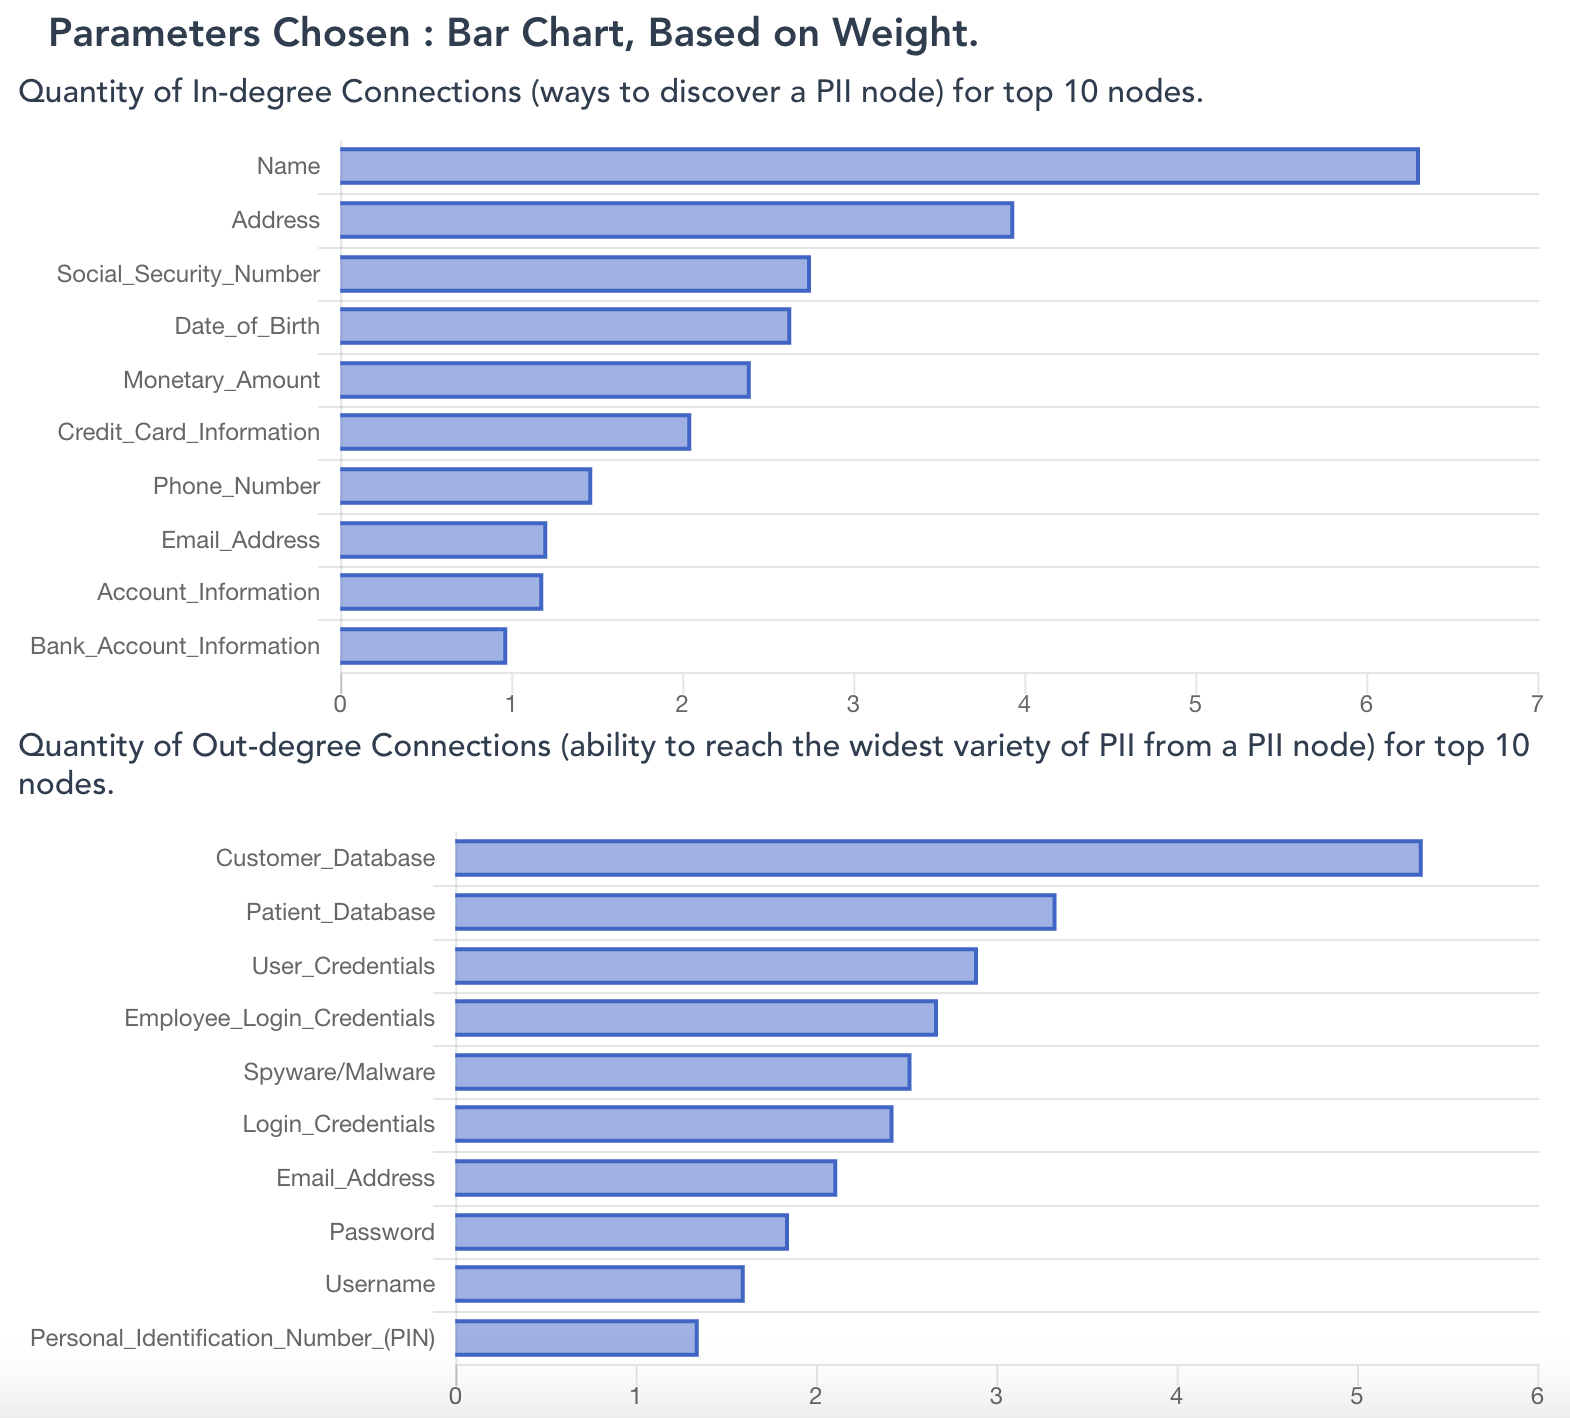
\includegraphics[width=\linewidth]{barchart_most_weight.png}
  \caption{A snapshot showing top 10 PII with most in and out probability sum on edges.}
  \label{fig:barchart_most_weight}
\end{figure}

\subsection{Statistical charts based on nodes}
\begin{itemize}
\item Distribution Chart based on node risk and value
\end{itemize}

We examine the distribution based on risk and value of each attributes to better understand the underlying trend for all properties. The chart is calculated by fixing linear interval size on x-axis and counting the number of PII lying in each interval. Figure~\ref{fig:node_value_distribution} gives a snapshot of the distribution chart for node value with interval unit of 100,000 in US Dollar value. According to the ITAP project\cite{ITAPDataSource}, ITAP determines the loss value of a PII  by averaging out the identity theft cases in which the PII was breached as a source of entry. Since ITAP usually lacks the number of victims involved in a case, the loss value is not per victim. Figure~\ref{fig:node_risk_distribution} yields a result for node risk with interval size 0.001.

{\bf Insight:} The vast majority of PII are valued at less than \$100,000 but have a risk of exposure of less than 0.001 too.

\begin{figure}[ht!]
  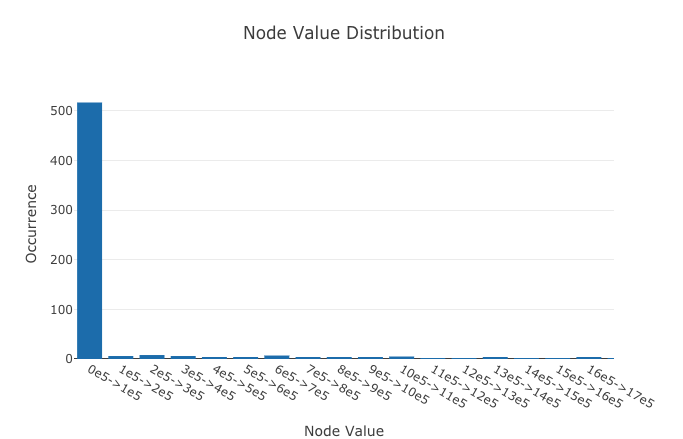
\includegraphics[width=\linewidth]{node_value_distribution.png}
  \caption{Distribution chart based on node value with interval size of \$100,000.}
  \label{fig:node_value_distribution}
\end{figure}

\begin{figure}[ht!]
  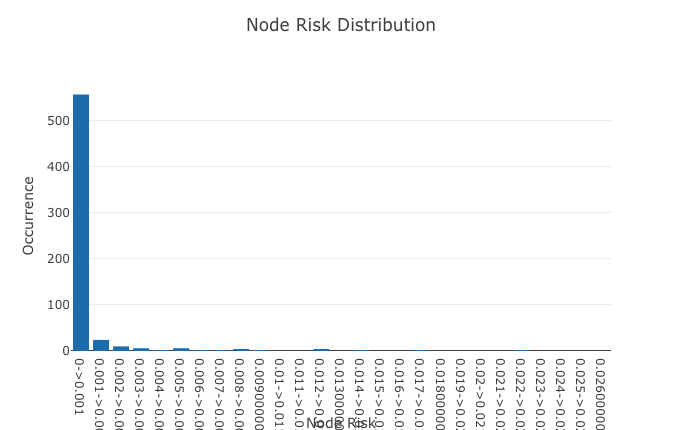
\includegraphics[width=\linewidth]{node_risk_distribution.png}
  \caption{Distribution chart based on node risk with interval size of 0.001.}
  \label{fig:node_risk_distribution}
\end{figure}

\begin{itemize}
\item Scatter plot of Closeness vs. Betweenness Centrality
\end{itemize}

Freeman \cite{Freeman78centralityin} developed a set of measures for centrality based on betweenness. Later on, he proposed four core criteria, which developed into degree, closeness, betweenness, and eigenvector centrality  \cite{Freeman79centralityin}. We further leverage the concept of closeness and betweenness centrality to investigate the Ecosystem graph.

\textbf{Closeness Centrality}
  emphasizes how close a vertex is to all other vertices in the topology -- the distance of a vertex to all others in the network by focusing on the geodesic measurement from each vertex to all others  \cite{Freeman79centralityin}. To be more specific, it calculates the shortest path between all nodes and assigns each node a score based on the length of its shortest paths to other nodes. According to Yin et al. \cite{Yin2006}, closeness is an evaluation for ``how long it will take information to spread from a given vertex to others in the network'' (p.1603), which helps find the PII attributes that are best placed to reach others once breached, and thus influence the entire network most efficiently. Consequently, closeness centrality in the identity ecosystem is a measure of {\bf Information Acquisition Power}. The highest it is for a PII attribute, the more power that PII attribute has in exploiting the entire identity ecosystem. Such PII attribute would only need few others to discover the whole network. Also according to Freidkin \cite{Freidkin}, closeness centrality represents the independence in the sense that PII attributes with higher closeness centrality do not need to seek information from other more peripheral PII attributes. 
This yields the equation as follows. $C_{c}(v_{i})$ stands for the closeness centrality for vertex $i$ and $\alpha (i, j)$ is the number of the shortest paths between two vertices $v_i$ and $v_j$ (considering the number of edges and not edge weight):
\begin{equation}
C_{c}(v_{i}) = \sum_{j = 1}^{n} \frac{1}{\alpha (i, j)}
\label{closeness_centrality_equation}
\end{equation}

\textbf{Betweenness Centrality}
Betweenness centrality  \cite{Freeman79centralityin} serves as an alternative concept of centrality focusing on control over the connections between other pairs of vertices. Betweenness centrality does this by identifying all the shortest paths and then aggregating how many times the node lies on one. Using $\alpha (i, j)$ as the number of different shortest $\langle i, j \rangle$ paths, and  $\alpha (i, u, j)$ as how many times the shortest path flows through $u$ ($ u \neq i, j$), the equation is as follows:
\begin{equation}
C_{B}(u) = \sum_{i \neq j \neq u}^{} \frac{\alpha (i, u, j) }{\alpha (i, j)}
\label{betweenness_centrality}
\end{equation}



Betweenness centrality recognizes nodes that act as `bridges' among whole and assesses the PII attributes that determine the flow around the system. Betweenness serves as a powerful characteristic for communication dynamics -- a high betweenness index could imply a node regulates collaboration in-between, holds authority over,  or infers periphery of diverse clusters. In our Ecosystem context, it measures how often a PII attribute is in the critical path of acquiring or discovering other PII, and hence measures {\bf Criticality}.




We calculate the scatter plot of Information Acquisition power (y-axis) vs. Criticality (x-axis).  This plot could further be divided into four quadrants based on the combination of high and low values on x and y axes. Denoting C for Criticality (i.e., betweenness) and I for  Information Acquisition Power (i.e., closeness), Figure~\ref{fig:scatterplot_hbhc} shows the graph with blue dots representing high C and high I, Figure~\ref{fig:scatterplot_lbhc} with green dots low C and High I, Figure~\ref{fig:scatterplot_hblc} with red dots High C and low I, and lastly Figure~\ref{fig:scatterplot_lblc} with orange dots low C and low I\footnote{Low and high are indicating below and above average, respectively.}. 

{\bf Insight:} Most of the data points maintain low information acquisition power and low criticality (Figure~\ref{fig:scatterplot_lblc}). There exists only few sparsely distributed data points, discussed in more details shortly, with both high criticality and high information acquisition power (Figure~\ref{fig:scatterplot_hbhc}). Such PII attributes are powerful in acquiring other PII and act as critical bottlenecks in the network of PII attributes. If evaluated using the Ecosystem model, these PII attributes could be asserted as attributes that will rapidly jeopardize the remaining sub-network if already exposed, and boost the information flow of exposure inside the system. Interestingly, there is only one data point with high criticality but low information acquisition power (Figure~\ref{fig:scatterplot_hblc}) and that is {\it Signature}.

\begin{figure}[ht!]
  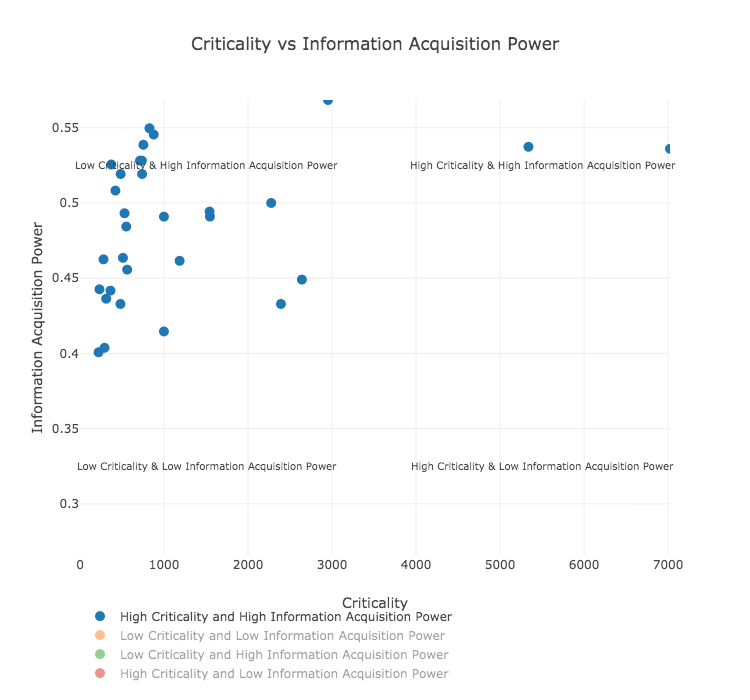
\includegraphics[width=\linewidth]{scatterplot_blue.png}
  \caption{Scatter plot with high betweenness (criticality) and high closeness (information acquisition power).}
  \label{fig:scatterplot_hbhc}
\end{figure}

\begin{figure}[ht!]
  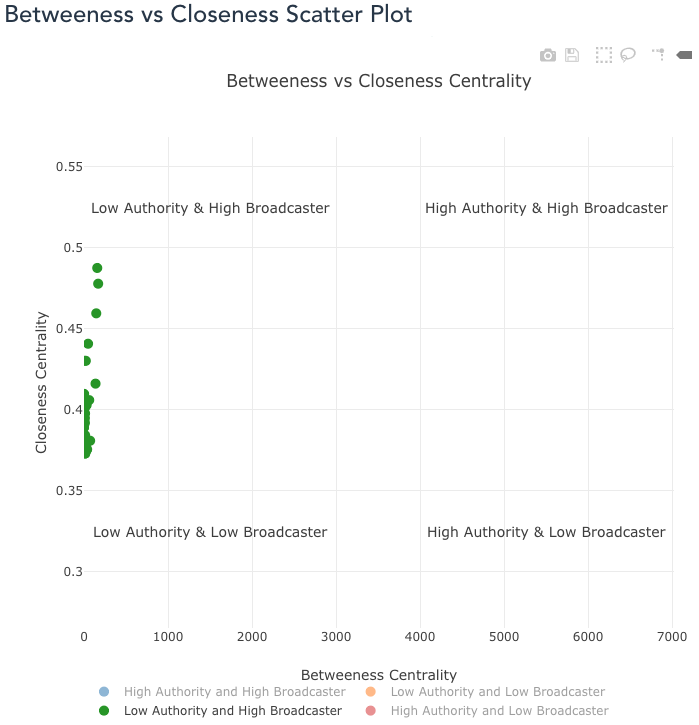
\includegraphics[width=\linewidth]{scatterplot_green.png}
  \caption{Scatter plot with low betweenness (criticality) and high closeness (information acquisition power).}
  \label{fig:scatterplot_lbhc}
\end{figure}

\begin{figure}[ht!]
  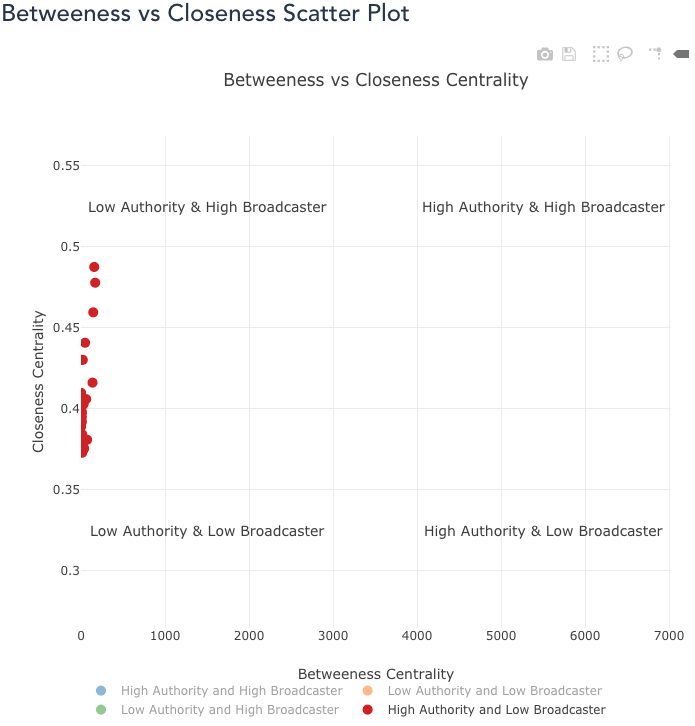
\includegraphics[width=\linewidth]{scatterplot_red.png}
  \caption{Scatter plot with high betweenness (criticality) and low closeness (information acquisition power).}
  \label{fig:scatterplot_hblc}
\end{figure}

\begin{figure}[ht!]
  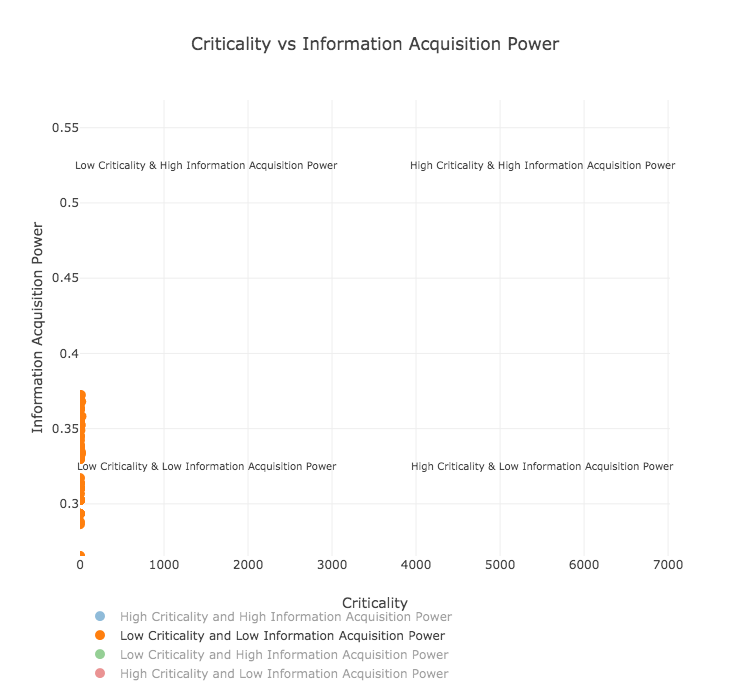
\includegraphics[width=\linewidth]{scatterplot_orange.png}
  \caption{Scatter plot with low betweenness (criticality) and low closeness (information acquisition power).}
  \label{fig:scatterplot_lblc}
\end{figure}


Figure~\ref{fig:top10_closeness_betweenness_centrality} displays the top 10 PII in descending order based on the value of information acquisition power and criticality.

{\bf Insight:} The top three attributes with the highest value of information acquisition power are \textit{Email Address}, \textit{Name}, and \textit{Address}. The top three attributes with the highest value of criticality are \textit{Customer Database}, \textit{Password}, and \textit{Email Address}. 

\begin{figure}[ht!]
  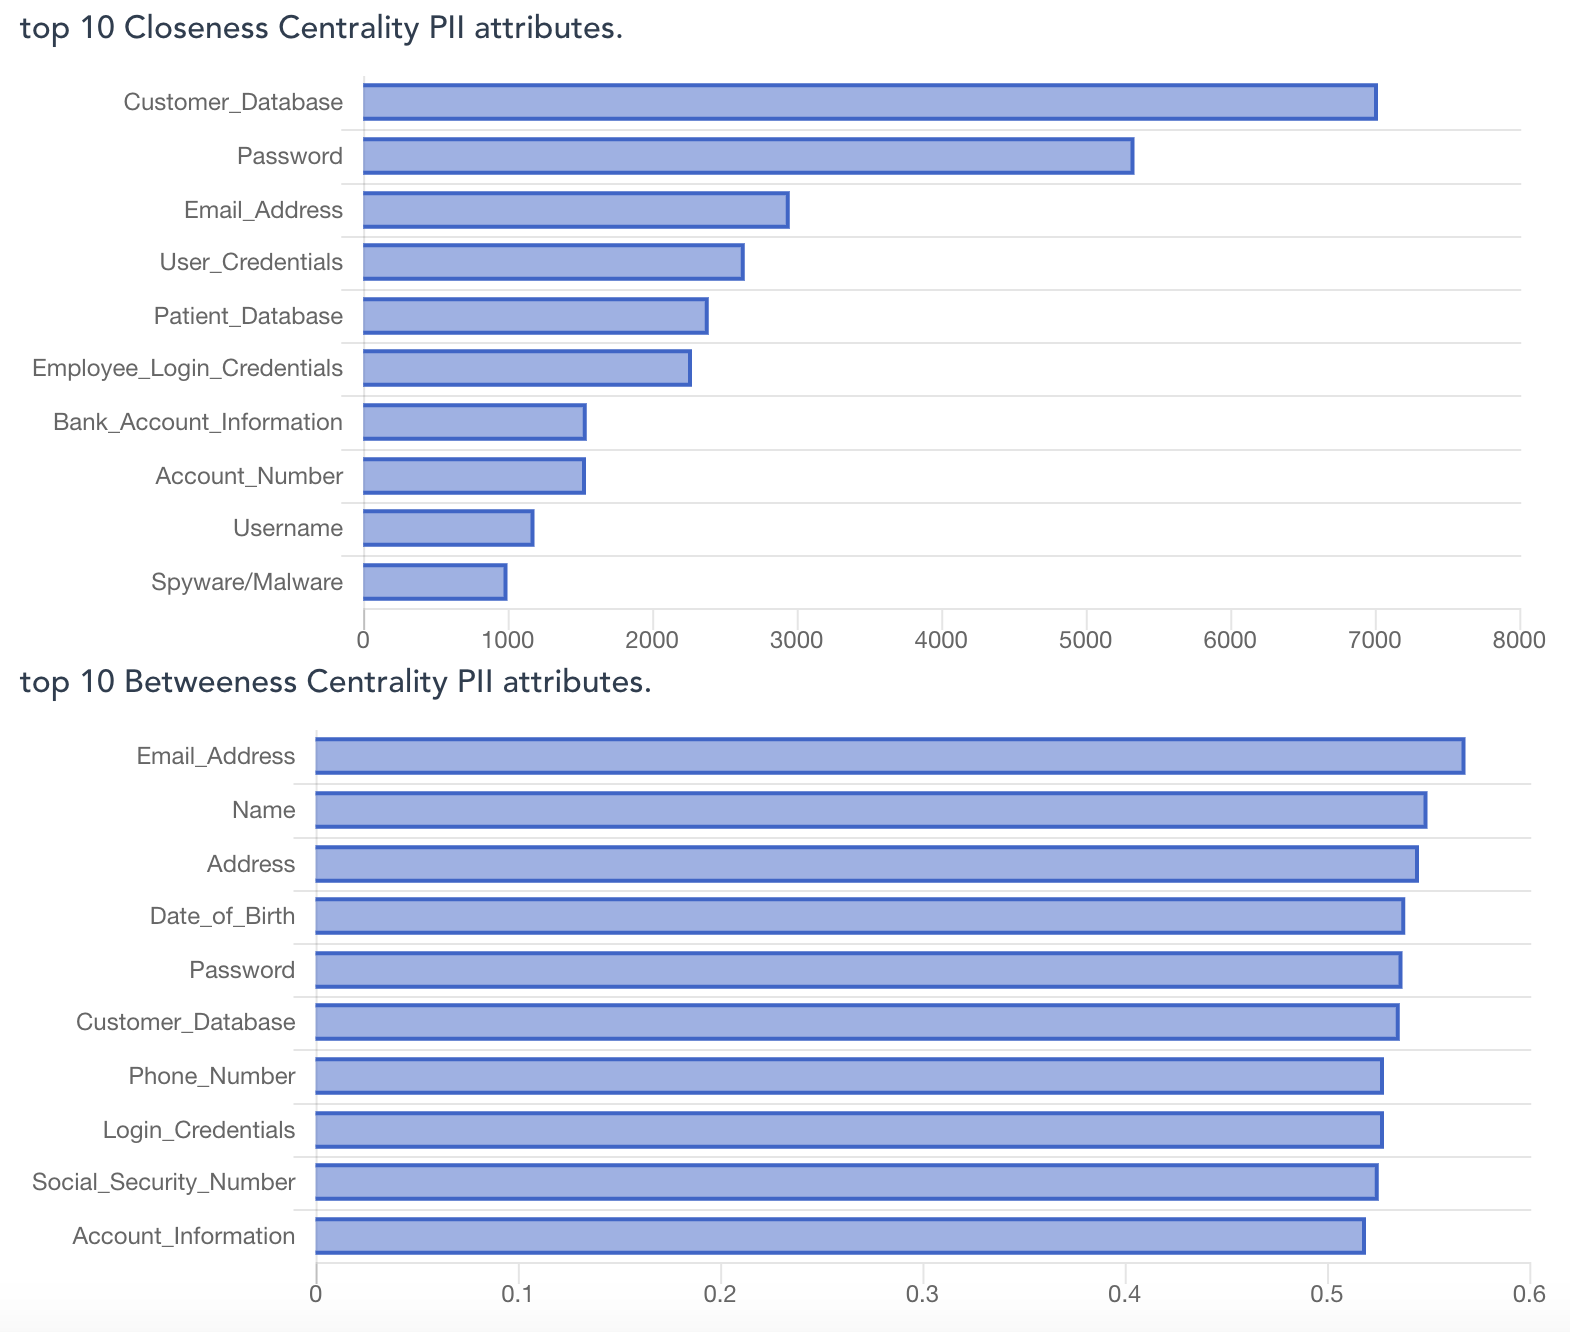
\includegraphics[width=\linewidth]{top10_closeness_betweenness_centrality.png}
  \caption{A snapshot showing  top  10  PII  with  highest information acquisition power and criticality values.}
  \label{fig:top10_closeness_betweenness_centrality}
\end{figure}

\subsection{Strongly Connected Components}
In the current Identity Ecosystem, a large portion (\%65) of nodes is completely isolated from the rest of the Ecosystem. Among those PII attributes with connections, we further identify attributes that are mutually coupled among themselves, which we define as `clusters'. Clusters serve as subsets that are dangerous sources for breaches, can quickly jeopardize other members in the group and confine the flow inside sub-network. 
We propose the cluster to be a Strongly Connected Component (SCC) in the graph theory. A SCC of a directed graph $G = (V, E)$ is a maximal set of vertices $U \subseteq V$ such that for every pair of vertices $u$ and $v$ in $U$, both $u \mapsto v$ and $v \mapsto u$ hold, where $u \mapsto v$ means there is a directed path from u to v. Consequently, in a cluster, there is a probability that every PII attribute can reveal every other PII and be revealed by every other PII. Tarjan's classic serial algorithm for detection of SCCs runs linearly with respect to the number of edges and uses depth-first search. We apply  Tarjan's algorithm \cite{Tarjan} to compute the clusters. We found one cluster of 36 nodes which we display in Table~\ref{table:1}.

{\bf Insight:} Every PII in Table~\ref{table:1} has a probability of exposing every other PII in that table. 

\begin{table*}[t!]
\centering
\begin{tabu} to 1\textwidth { | X[l] | X[l] | X[l] | }
    \hline
    \multicolumn{3}{|c|}{Cluster of attributes, containing 36 vertices  sorted in alphabetical order.} \\
    \hline
    1. Address & 2. AccountNumber & 3. AccountInformation \\
    \hline
    4. Age & 5. BankAccountInformation & 6. BankAccountNumber \\
    \hline
    7. BiographicData & 8. BirthCertificateInformation & 9. CreditCardInformation \\
    \hline
    10. CreditCardNumber & 11. CVVCode & 12. CheckInformation \\
    \hline
    13. DateofBirth & 14. DebitCardInformation & 15. Driver'sLicenseNumber \\
    \hline
    16. Driver'sLicenseInformation & 17. Date & 18. EmployeeLoginCredentials \\
    \hline
    19. EmailAddress & 20. EmployeeRecord & 21. ExpirationDate \\
    \hline
    22. IDCardInformation & 23. LoginCredentials & 24. Name \\
    \hline
    25. Password & 26. PersonallyIdentifiableInformation & 27. PhoneNumber \\
    \hline
    28. PersonalIdentificationNumber(PIN) & 29. PhysicalAddress & 30. PassportInformation \\
    \hline
    31. Photograph-Person & 32. PatientMedicalRecord & 33. RoutingNumber \\
    \hline
    34. SocialSecurityNumber & 35. Username & 36. W-2FormInformation \\
    \hline

\end{tabu}
\caption{List of attributes in SCC.}
\label{table:1}
\end{table*}

\section{Discussion of Results}

In this section, we analyze the statistical results and give example takeaways from the above charts. Overall the Ecosystem contains 627 vertices. We can observe that a large portion of the nodes is not connected to any other node.  In fact,  65\% of the nodes are fully isolated without any inbound or outbound  connections.  Only a small portion is considered to be important when breached or compromised, and one should make an effort to protect them. Among those with connections, we further observe the ranking by degree centrality to speculate candidates with most in-degree versus most out-degree, which could be interpreted as attributes that are most likely to get compromised, versus attributes that tend to spread information. 

We further discover possible layout and structural features for the Identity Ecosystem graph by computing the SCC of the network. We extracted clusters, wherein each node is inter-reachable inside the sub-graph. Between that 33\% with incoming and 7\% with outgoing edge PII nodes, an overlap of 36 (about 5\%) vertices constitutes a big component. 

We can assert our ecosystem model to be a sparse graph, where most attributes are unreachable. Only 5\% congregate together and serves as a central concern for our identity management.

We utilized closeness and betweenness centrality to better understand the influence in the topology.  Closeness, or information acquisition power in this context,  measures the ability of a PII attribute to retrieve information from and send information to others. Those PII attributes with high value can be viewed as `broadcaster' or `gossiper', which if breached, can put others in danger. Betweenness, or criticality in this context, is based on the assumption that a PII attribute may be exposing others if it presides over a path bottleneck. It also identifies the boundary spanner, which separates different communities and features. Those PII attributes with high value can be viewed as `bridge' or `broker', if one connecting component is breached, those can function as essential endpoints to protect the identity by not allowing information to flow through. 

Generally, previous studies indicate that centrality metrics are positively correlated \cite{Correlated} \cite{CorrelationCoefficient}. 
Overall degree and closeness were strongly inter-correlated, while betweenness remained relatively uncorrelated with the other measures \cite{Bolland}. Combinations of centrality values represent certain topology and positional patterns (\cite{Donglei} p. 51). Given attributes with high degree and low closeness centrality (information acquisition power), we can assert that the PII is embedded in the cluster and far away from others, whereas low betweenness (criticality) infers that the PII holds redundant links where information just bypass it. Given attributes with a low degree and high closeness centrality (information acquisition power), the PII ties with substantial or active others, whereas high betweenness (criticality) indicates that PII is spanning few links, but with crucial influence on network flow. Low closeness (information acquisition power) and high betweenness (criticality) combination results in specific PII monopolizing the ties from a small number of PII attributes to many others. We found a  prime example of such situation with {\it Signature}. Low betweenness (criticality) and high closeness (information acquisition power) portray the PII locates in a dense, active cluster at the center of events with many others. We summarize different combinations and their corresponding characteristics in Table~\ref{table:2}.

\begin{table*}[t!]
\centering
\begin{tabular}{ |p{4cm}||p{4cm}|p{4cm}|p{4cm}|  }
 \hline
    & Low Degree & Low Closeness (Information Acquisition Power) & Low Betweenness (Criticality)\\
 \hline
 High Degree   & -    & Embed in a cluster which is faraway from others & PII with redundant connection - flow bypass \\
 \hline
 High Closeness (Information Acquisition Power) &   Key PII connected to important and active others  & -   & Center PII located  in  a  dense,  active cluster at the center of events with many others \\
 \hline
 High Betweenness (Criticality) & PII's few ties are crucial to network flow &  PII monopolizes
the ties from a small number of PII to many others  &  - \\
 \hline
\end{tabular}
\caption{Combinations of centrality metrics.}
\label{table:2}
\end{table*}

\section{Related Work}

In this section, we cover previous research that studies and surveys the statistics of identity theft. We can categorize previous work into three main sources: Federal and States agencies, private organizations and academic institutions.

From government sources, Federal and State agencies, studies by U.S. department of Justice (Harrell \cite{Harrell}) release reports on distribution of identity theft victims. Also United States General Accounting Office (USGAO \cite{USGAO}), Federal Trade Commission (FTC \cite{FTC}), Office of the Inspector General, Federal Bureau of Investigation (FBI), Postal Inspectors Office, and United States Secret Service (USSS) present studies on identity theft from different domains. 

Among private organizations, Javelin \cite{Pascual} publishes comprehensive analysis and case studies about fraud detection and identity threat.

In the academia, Copes et al. \cite{Copes} analyzed reports from National Public Survey on White Collar Crime and summarized financial-related fraudster behavior such as credit card fraud and bank account fraud. Allison et al. \cite{Allison} gathered data from agencies. They performed statistics analysis on victims and extracted demographic patterns of victims among the general U.S. population. Using Routine Activity Theory, Reyns \cite{Reyns} reported an empirical study of identity theft in the United Kingdom. Pratt et al.\cite{Pratt}, and Choo, \cite{Choo} also conducted studies utilizing Routine Activity Theory in different jurisdictions. 

 
In these studies, statistic were presented. However, those data sets were not fully constructed into a structured mathematical model and do not interact with graph theoretic and social network analysis measures. We feed data sets from ITAP and model the risk of exposure using Bayesian Network \cite{EcosystemModeling}. We are also one of the first to develop identity ecosystem into graph network and exploit the concept from three types of centrality as well as strongly connected components.  

\section{Conclusion}

In this paper, we designed and implemented a visualization framework that assists data providers and collectors to comprehend and analyze the probabilistic graphical model of identity attributes. The visualization tool facilitates understanding of the whole risk model. Based on the Bayesian network presentation of identity attributes, we developed traditional statistical charts such as histograms, scatter plots, and pie charts based on values for each PII to inspect the underlying distribution. Even though hundreds of PII constitute the whole system, a large amount is indeed isolated. Only a small portion of the PII is vulnerable to identity theft and one should make an effort to protect them.

To investigate the structural topology and correlation between PII, we further proposed to apply centrality measures such as degree, closeness, and betweenness centrality. Moreover,  we discussed the combination of all the three centrality measures with high and low values. With these measures, we can estimate the hidden characteristics of the network.

Lastly, we calculated Strongly Connected Components (SCC) to recognize clusters of PII that are mutually reachable among themselves.  SCCs are subsets which are dangerous origins for breaches, can quickly jeopardize other PII in the group and constraint the flow inside the sub-network. In the current Identity Ecosystem, there is only one big cluster with 36 PII (5\% of the entire ecosystem) interconnected. We can again confirm  that as complex as the Identity Ecosystem is, a small portion is considered most threatening and risky. 

As the ITAP project continues to collect data, theories and technologies developed from this research can be customized along the way to minimize our identities'  risk of exposure and maximize privacy.


%\section{Acknowledgments}

%We wish to thank the Center for Identity Partners (\url{https://identity.utexas.edu/strategic-partners}) for their contributions to this research effort.

%\section{Appendices}
%
% The acknowledgments section is defined using the "acks" environment (and NOT an unnumbered section). This ensures
% the proper identification of the section in the article metadata, and the consistent spelling of the heading.
% \begin{acks}
% To Robert, for the bagels and explaining CMYK and color spaces.
% \end{acks}

%
% The next two lines define the bibliography style to be used, and the bibliography file.
\bibliographystyle{IEEEtran}
\bibliography{IEEEabrv,sample-base}

% 
% If your work has an appendix, this is the place to put it.
\appendix

\end{document}
